% This version of CVPR template is provided by Ming-Ming Cheng.
% Please leave an issue if you found a bug:
% https://github.com/MCG-NKU/CVPR_Template.

%\documentclass[review]{cvpr}
\documentclass[final]{cvpr}

\usepackage{lipsum}  


\usepackage{times}
\usepackage{epsfig}
\usepackage{graphicx}
\usepackage{amsmath,bm}
\usepackage{amssymb}
\usepackage{booktabs}

% Include other packages here, before hyperref.

% If you comment hyperref and then uncomment it, you should delete
% egpaper.aux before re-running latex.  (Or just hit 'q' on the first latex
% run, let it finish, and you should be clear).
\usepackage[pagebackref=true,breaklinks=true,colorlinks,bookmarks=false]{hyperref}


\def\cvprPaperID{****} % *** Enter the CVPR Paper ID here
\def\confYear{CVPR 2021}
%\setcounter{page}{4321} % For final version only


\begin{document}

%%%%%%%%% TITLE
\title{Deep learning for hand prosthesis piloting based on sEMG signals}

\author{Benady Antoine\\
Master MVA\\
École normale supérieure Paris-Saclay\\
{\tt\small antoine.benady@ens-paris-saclay.fr}
% For a paper whose authors are all at the same institution,
% omit the following lines up until the closing ``}''.
% Additional authors and addresses can be added with ``\and'',
% just like the second author.
% To save space, use either the email address or home page, not both
\and
Reme Raphaël\\
Master MVA\\
Institut Polytechnique de Paris\\
{\tt\small raphael.reme@telecom-paris.fr}
}

\maketitle

%%%%%%%%% ABSTRACT
\begin{abstract}
  The development of comfortable hand prosthesis is still an open challenge. The question of retrieving the user's intentions is limiting in this design. Over the past few years, research has shown that the exploitation of electromyographic signals (sEMG) is promising. Recent advances in deep learning have opened up new perspectives for predicting user intent from sEMG signals. Our work focuses on the use of recursive neural networks (RNN) to predict the position of each hand angle from sEMG signals. 
  We implemented architecture inspired from literature based on LSTM cells (Long-Short Terms Memory). 
 We also take the initiative to extend these architectures to GRU (Gated recurrent unit) and to introduce new loss functions.
 
\end{abstract}
%%%%%%%%% BODY TEXT

\section{Introduction}
%/Motivation/Problem-Definition. 15\%

Active, handy and cheap hand prosthesis conception is currently a challenge. It’s limited by the complexity of the movements of the human hands, and by the interpretation of the user’s will. This challenge can have important repercussions on the lives of amputees of superior limb.\\

In the context of upper limb prosthesis design, one main difficulty remains the implementation of the human-machine interface. For years, the state-of-the-art has focused on the search for a solution to acquire the user's intention. The problem is often stated as a classification problem \cite{classification}, where the goal is to find the movement desired by the user among a set of gestures and then execute it. But this formulation of the problem is really limited by the number of gestures considered, and does not grant an intuitive control over the prosthesis. Some recent results seem to show that, with the recent breakthroughs in deep learning, the regression problem could be addressed \cite{Koch} (guessing directly all the relative positions of the hand from the user’s will). It brings a much more intuitive control over the prosthesis and is not limited by a set of pre-defined gestures, which would significantly improve the comfort of people with prostheses.

To date, the most promising technique remains the processing of electromyographic signals. Surface electromyographic electrodes (sEMG) measuring a set of muscle-activating action potentials are widely used in research. They have the advantage of being non-invasive, easy to set up, and they have made it possible to develop many motion classification algorithms.\\

Here, we focused on the regression problem. The problem can be addressed as the following : given a signal $\pmb{x}_t \in \mathbb{R}^d$, where $d$ is the number of electromyographic sensors, we would like to predict, the more accurate as possible, the 22 \footnote{or 18, depending on the database used} hand joint coordinates signal $\hat{\pmb{y}}_t \in \mathbb{R}^{22}$. We have several databases from the Ninapro projects \cite{database} providing us $\pmb{x}_t$ and the ground truth ${\pmb{y}}_t$ hand motion. The Ninapro databases gather several subjects that have been asked to reproduce a motion projected on a screen. The electromyographic (EMG) sensors and a glove provide respectively the EMG and the 22  hand joint coordinates. The goal is to minimize the mean absolute error (MAE). The general framework is illustrated figure \ref{general_framework}, and figure \ref{hand} shows the position of the hand joint coordinates.


%\textcolor{red}{\textit{Introduce notation, provide formal definitions as needed, define any
%constraints or restrictions, define what you try to solve/optimize (e.g., maximize or minimize an optimization function, or the accuracy of an algorithm). Describe the problem in a formal way. Describe the hardness of the problem in a formal way.} }

%
\begin{figure}[t]
	\begin{center}
		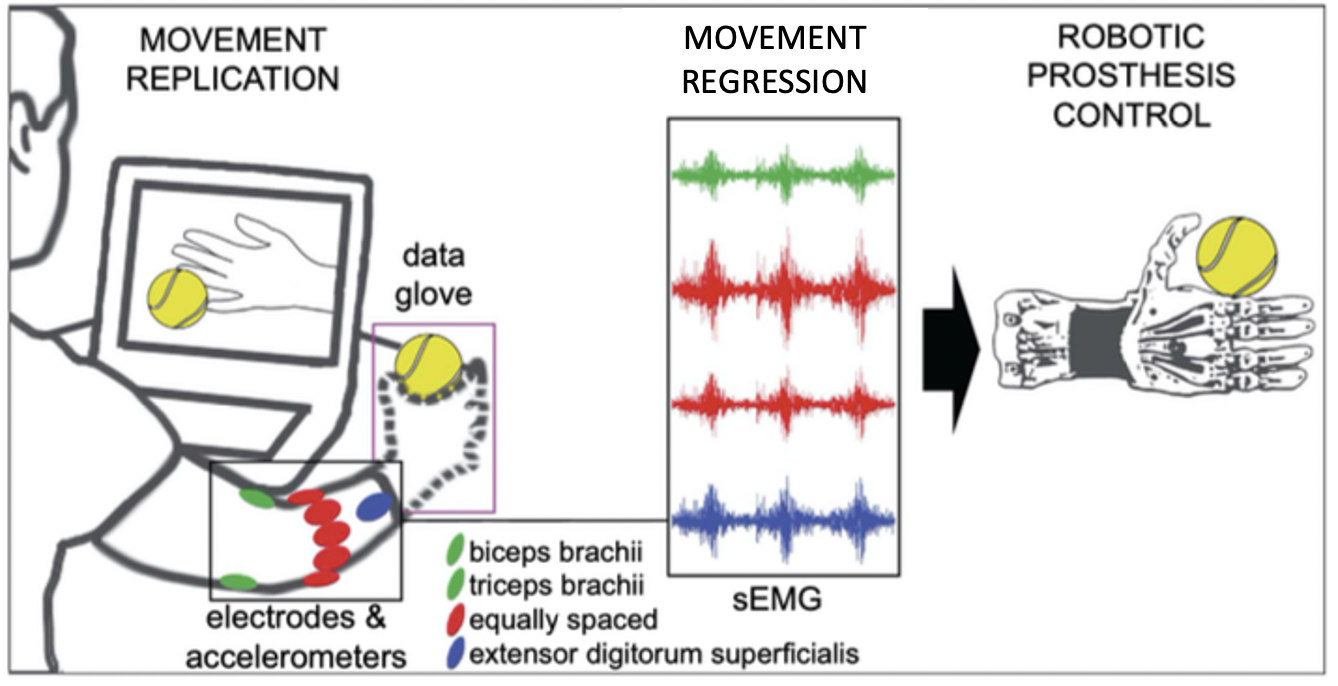
\includegraphics[width=0.9\linewidth]{framework}
	\end{center}
	\caption{General framework of the project. This article focus on the movement regression task}
	\label{general_framework}
\end{figure}

\begin{figure}[t]
	\begin{center}
		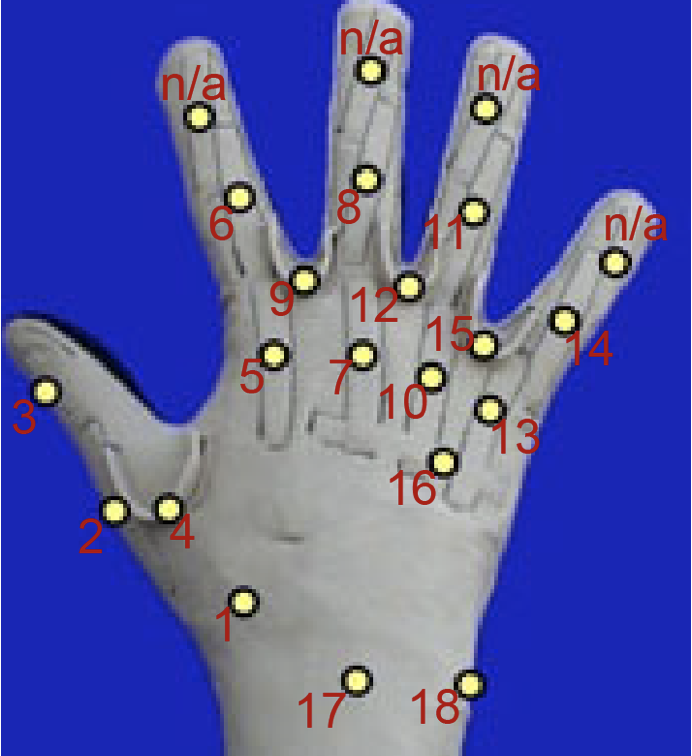
\includegraphics[width=0.5\linewidth]{hand.png}
	\end{center}
	\caption{Position of the hand joint coordinates (for database VII). Credit \cite{Krasoulis2017}}
	\label{hand}
\end{figure}


\section{Related work.}
The question of predicting the user's intention was initially stated as a classification problem. The goal was to predict the intention of the user among predefined postures. Before the emergence of deep learning, a challenge was to extract relevant features for classification \cite{Features_extraction}. Phinyomark et al. distinguish four main types of method for features extraction : energy and complexity, frequency, prediction model, and time-dependence. \\

Then, deep learning based methods achieve similar results \cite{coteallard2019deep,Ding_2018} as the previous methods. Indeed, feature extraction is included in the learning in the first layers of the networks.\\

However, the classification problem has a main inconvenient: the output motion is limited among a set of postures, which is restrictive for amputees daily life. With the growth of databases size and improvement of deep learning techniques, regression problem seems now achievable \cite{Kir,Koch,Quivira}. Both Hoch et al. and Quivra et al. achieve promising results for this problem. \cite{Kir,Koch,Quivira} use recurrent neural networks to tackle the regression problem.

In this article, we focus on the regression problem with recurrent neural networks as well.

\section{Methodology}
This section present our methodology. In the first place, information on the database are provided. Secondly, the splitting strategy used. Thirdly pre-processing techniques such as sub-sampling, normalization and standardization are introduced. Then, we present our model which is based on LSTM. In the last part, we present the training process.
\subsection{Database}
The first step of our project was to find a good database. A quick literature review told us that the Ninapro databases are the references in the field. We had to choose among the different databases from the Ninapro project. A PhD student told us that the recent databases are more accurate than the first ones. Then we read in \cite{Koch}, that the best results were obtained using the database VII so that's the one we chose.
Before the pre-processing, we have access to the Ninapro database VII defined in \cite{Krasoulis2017}. Table \ref{database_info} summarizes information on these databases.

\begin{table}
	\begin{center}
		\begin{tabular}{l c  }
			\toprule
			 & Ninapro DB VII \\
			\hline
			Number of subjects & $20^\star$   \\
			Number of EMG sensors & 12  \\
			Number of joint coordinates  & 18 \\
			Sampling frequency & 2kHz  \\
			Size (Gb) & 33  \\
			\toprule
		\end{tabular}
	\end{center}
	\caption{Information on the database, before pre-processing.\\
	\emph{$\star$ We haven't not use the 2 amputees as the hand movements are not recorded.}}
	\label{database_info}
\end{table}

\subsection{Database splitting}
For our experiments, we have split our dataset in subsets in order to validate our method. The idea is to train the network on the "train subset", validate our different trainings on the "validation subset" and test our final model on the "test subset".

We have split the dataset along subjects. The goal is to train on some subjects and evaluate the model on other subjects. In the end we would like to have a single model able to handle any new subject.

This is particularly useful for amputees as we cannot train the model on them as we do not have the regression data.

In order to reduce bias we have split the 20 subjects of the database in three subsets keeping the left handed ratio as constant as possible (We used the meta information provided by Ninapro).


\paragraph*{Split sequences}A ENLEVER!! In this process we train on all the users of the database. But only on some parts of their exercise. And we validate and test on other parts. It should be an easier task but it's much less useful for our goal.

We made sure not to use overlapping sequences on training and testing, and in order to avoid to add bias to the subsets, we split all the exercise of each subject in the different subsets.

\subsection{Pre-processing}
Table \ref{database_info} highlights the important size of the database. In order to allow fast computations, sub-sampling is needed to deal with the quantity of data. A trade-off has to be found between fast computation and loss of information. A sub-sampling at 400Hz was carried out, the results of which can be seen in figure \ref{sub-sampling}. \\

The ranges of variation of sEMG measurements vary greatly from one sensor to another, which can be a problem during training with LSTM (long-short term memory) cells. To address this issue, normalization or standardization are used on the each input $\pmb{x}_{i}$.
The normalization operation can be stated as :
$$\forall t \; x_{t,i,norm}=\frac{x_{t,i}-x_{i,min}}{x_{i,max}-y_{i,min}}$$
where $x_{i,min}$ and $x_{i,max}$ are respectively the minimum and the maximum of each input on the whole database.

The standardization operation can be stated as :

$$\forall t \; x_{t,i,stand}=\frac{x_{t,i}-\bar{x}_{i}}{\sigma_i}$$
where $\bar{x}_{i}$ and $\sigma_i$ are respectively the mean and the standard deviation of each input on the whole database. In our project, the standardization process gave better results so this is the one we kept for the following.

\begin{figure}[t]
	\begin{center}
		%\fbox{\rule{0pt}{2in} \rule{0.9\linewidth}{0pt}}
		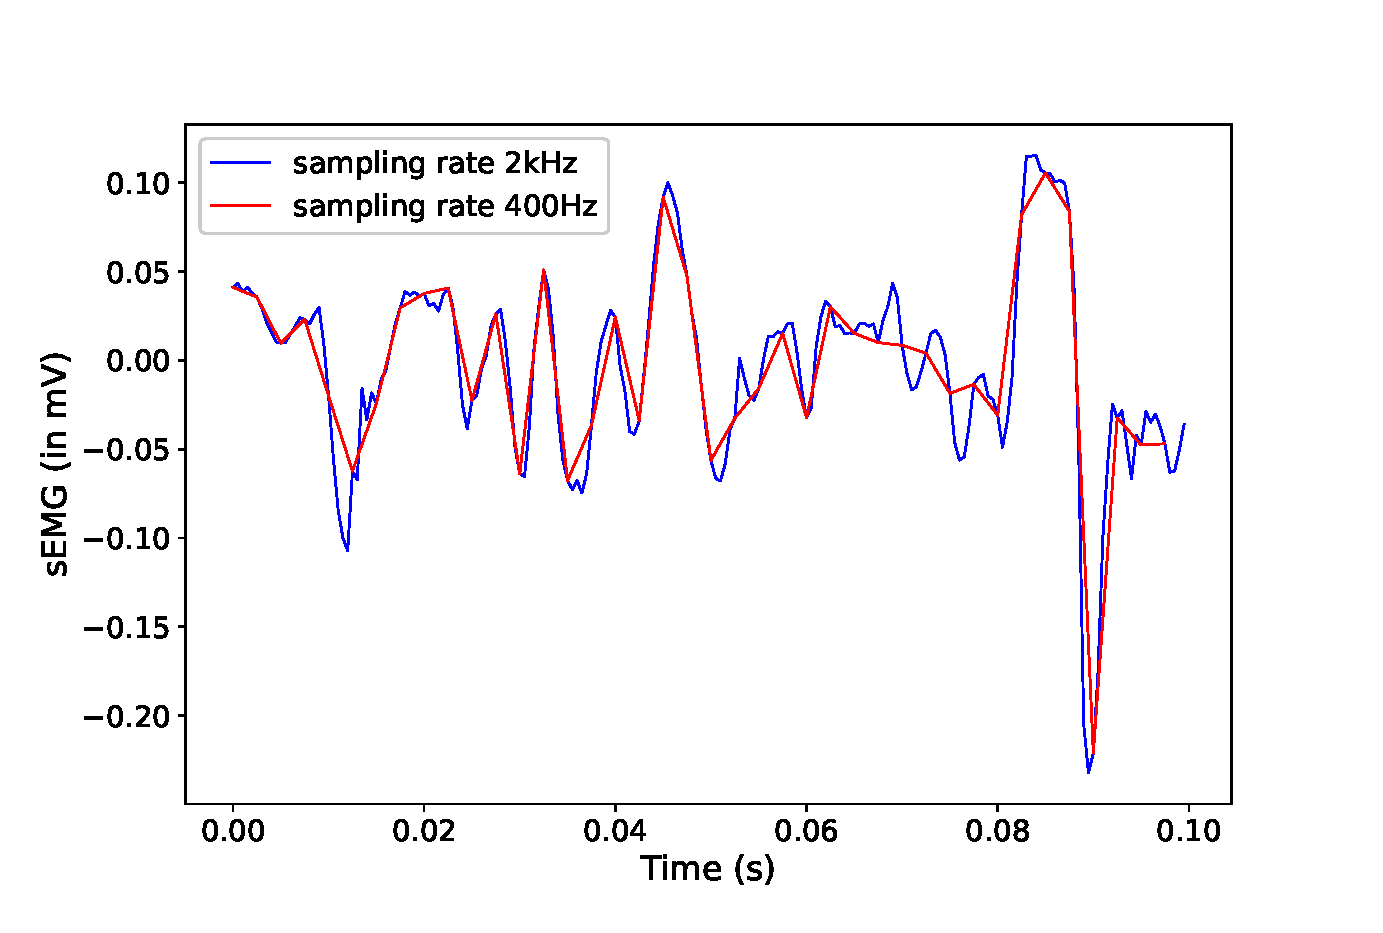
\includegraphics[width=\linewidth]{subsampling.eps}
	\end{center}
	\caption{Influence of the sub-sampling at 400Hz on one sEMG signal}
	\label{sub-sampling}
\end{figure}
 
\subsection{Model}

We used two types of recurrent neural network (RNN) architectures. The first one is based on LSTM cell and the second one is based on GRU (gated recurrent unit) cell. We describe these cells in the following paragraphs.
\subsubsection*{LSTM cell}
Figure \ref{LSTM} shows the general principle of a LSTM cell. With $\pmb{x}$ one element of an input sequence, $\pmb{h}$ / $\pmb{c}$ the corresponding output / hidden sate. The update of the cell is given by : \\
$$\pmb{c}_t=\pmb{f}_t\odot \pmb{c}_{t-1}+\pmb{i}_t\odot\tanh(\pmb{W}_{xc}\pmb{x}_t+\pmb{W}_{hc}\pmb{h}_{t-1}+\pmb{b}_c)$$
With $\odot$ being the Hadamard product, with the input gate :
$$\pmb{i}_t=\sigma(\pmb{W}_{xi}\pmb{x}_t+\pmb{W}_{hi}\pmb{h}_{t-1}+\pmb{b}_i)$$
and the forget gate :
$$\pmb{f}_t=\sigma(\pmb{W}_{xf}\pmb{x}_t+\pmb{W}_{hf}\pmb{h}_{t-1}+\pmb{b}_f)$$
The output of the LSTM cell is described by : 
$$\pmb{h}_t=(\pmb{W}_{xo}\pmb{x}_t+\pmb{W}_{ho}\pmb{h}_{t-1}+\pmb{b}_o)\odot\tanh(\pmb{c}_t)$$

All the $\pmb{W}$ are trainable weights and $\pmb{b}$ bias terms
.

\begin{figure}[t]
	\begin{center}
		%\fbox{\rule{0pt}{2in} \rule{0.9\linewidth}{0pt}}
		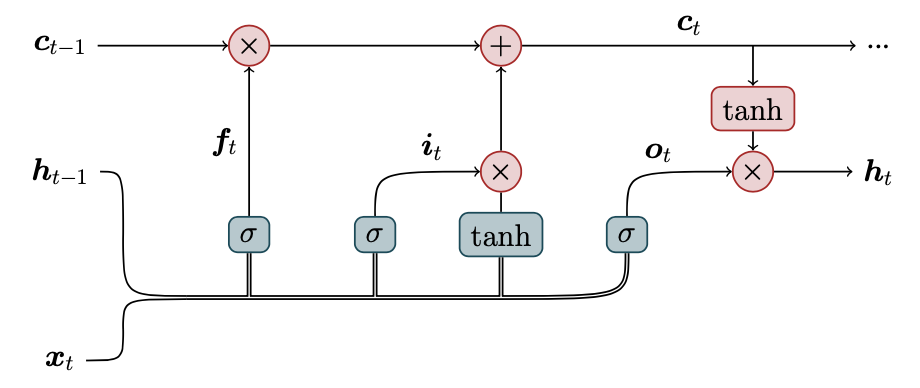
\includegraphics[width=0.95\linewidth]{LSTM_cell}
	\end{center}
	\caption{Illustration of the principle of a LSTM cell. Credit \cite{Koch}}
	\label{LSTM}
\end{figure}

\subsubsection*{GRU cell}
Figure \ref{GRU} shows the general principle of a GRU cell. The output of the cell is given by : 
$$\pmb{h}_t=(1-\pmb{z}_t)\odot{\pmb{h}_{t-1}}+\pmb{z}_t\odot{\tilde{\pmb{h}}_{t}}$$

With : 
$$\pmb{z}_t=\sigma(\pmb{W}_z\cdot[\pmb{h}_{t-1},\pmb{x}_t])$$
$$\pmb{r}_t=\sigma(\pmb{W}_z\cdot[\pmb{h}_{t-1},\pmb{x}_t])$$
$$\tilde{\pmb{h}}_t=\tanh(\pmb{W}[\pmb{r}_t\odot\pmb{h}_{t-1}),\pmb{x}_t])$$
Where $\pmb{W}$ are all training weights.

\begin{figure}[t]
	\begin{center}
		%\fbox{\rule{0pt}{2in} \rule{0.9\linewidth}{0pt}}
		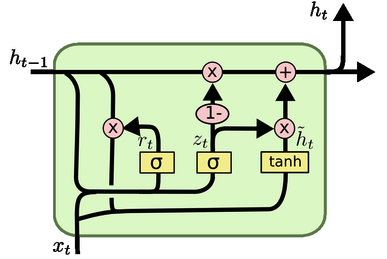
\includegraphics[width=0.95\linewidth]{GRU}
	\end{center}
	\caption{Illustration of the principle of a GRU cell. Credit \cite{GRU}}
	\label{GRU}
\end{figure}

\subsubsection*{Architectures}
We implemented several architectures based on LSTM and GRU. Table \ref{architectures} details the best architectures we used for LSTM and GRU cells.
\begin{table}
	\begin{center}
		\begin{tabular}{l c c }
			\toprule
			& Architecture 1 & Architecture 2 \\
			\hline
			Cell type & "GRU" & "LSTM"   \\
			Input dimension & 12 & 12 \\
			Hidden dimension & 128 & 128 \\
			Number of layers & 1& 1\\
			\hline
			Fully-connected  & 128 x 18& 128 x 18\\
			\toprule
		\end{tabular}
	\end{center}
	\caption{Descriptions of the architectures used.}
	\label{architectures}
\end{table}

\subsection{Training process}

At training time, we extract all the sub-sequences $\{(x_k, y_k)_{i \le k<i+L}, i\}$ of fixed length L in our training subset and train over each of them in order to leverage all the information of the dataset. We used $L=400$ in order have 1s length sequences as in \cite{Koch}.

We use RNN over these sequences in a sequence to sequence way, in order to predict all the targets of each sequence. At each epoch we validate the model as describe in \ref{section:evaluation}.

Our main contribution compared to the articles we read is the work on the training loss function. First we started by using the Mean Square Error (MSE) function over the whole sequence: 
$$\mathcal{L}(Y,\hat{Y})=\frac{1}{n}\sum (Y-\hat{Y})^2$$
Where $n$ is the number of joint angles multiply by the length of a sequence.
Yet, one particularity of the dataset is that during the exercises the subjects are "resting" most of the times, \textit{i.e.} there is no movement. Therefore, during the process our network learnt to predict a constant around the mean for each joint coordinates and seems to struggle to go beyond (It requires more epochs to do so.)

In order to improve things we worked on the loss function. First rather than using a MSE loss over the whole sequence we tried to use a MSE loss only over the last target of the sequence. (Using MSE loss over the whole sequence is probably to hard, as the network has not enough information to predict the angles at the beginning of the sequence.).

We also designed a new loss in order to focus on what we want to learn: Movement.
This loss will perform a weighted MSE loss over the sequence. First it will apply a decay factor, the idea is to allow the first predictions to be wrong, and to mainly focus on the end of the sequence. And second, it will also apply a multiplicative factor according to the current derivative of the angle movements at this time step.

Our loss function can be stated as the following :
\begin{equation*}
    \begin{aligned}
        \mathcal{L}(Y,\hat{Y})= \sum_{t=1}^L \alpha_t \beta_t(Y) (Y_t - \hat{Y}_t)^2
    \end{aligned}
\end{equation*}

Where $\alpha_t$ is an increasing function of $t$. We typically used $\alpha_t = \frac{t^p}{L}$ with $p$ a parameter to tune.

And $\beta_t(Y)$ is an increasing function the absolute difference between $Y_t$ and $Y_{t-1}$ (The movement at time $t$). We used $\beta_t(Y) \propto \epsilon + |Y_t - Y_{t-1}|^q$ where $q$ and $\epsilon$ are parameters to tune.

In order to keep meaningful losses we averaged all the losses by the batch size, sequence length and positions numbers, with these settings we use a batch size of 256, with Adam optimizer and a learning rate of 0.001.

\section{Evaluation and results}
\subsection{Evaluation}
\label{section:evaluation}
We decided to evaluate the performance of our model like the papers \cite{Koch,Kir,Quivira} to enable comparison, although the database are not always the same. We used the mean absolute error (MAE): 
$$MAE(Y,\hat{Y})=\frac{1}{n}\sum |Y-\hat{Y}|$$

After each epoch of training, we evaluate the performances over the validation set with the MAE loss. At validation time, we use each exercise as a single very long sequence: The MAE over a real long sequence seems a better metric than the MAE over the artificial sub-sequences.

Moreover as we noticed, the network is struggling to predict anything but an approximation of the mean. We have therefore decided to create a baseline predictor: The mean predictor. We have computed the mean of the joint angles over the training set. And predict for the validation/test sets these means. The computation of the associated MAE loss will be our baseline. And our goal is to improve this prediction, and as we will saw this is not easy at all.


\subsection{Results}
\subsection*{Influence of the architecture}
First, we focused on the choice of the architecture. AS GRU cells are relatively news compared to LSTM, all the articles \cite{Koch, Quivira, Kir}  we read were based on LSTM. Therefore we compared GRU and LSTM based architectures. GRU are reputed to increase the speed of the training. We confirmed this reputation but yet the training was less performing when we look closer at the validation loss as we can see table  \ref{GRUvsLSTM}


\begin{table}
	\begin{center}
		\begin{tabular}{l c c }
			\toprule
			& Arch. 1 & Arch. 2 \\
			\hline
			Duration of 1 training epoch & 1208s & 1290s   \\
			Validation loss after 1 epoch & 16,24 & 14,95 \\
			\toprule
		\end{tabular}
	\end{center}
	\caption{Performances during training of architecture 1 and 2 (defined table \ref{architectures})}
	\label{GRUvsLSTM}
\end{table}

\subsection*{Influence of the loss function}

We did a lot of experiments to find out how to learn efficiently. We never really managed to do better on the validation set than the mean baseline. And it seems that the same problem occurs in the literature: Those who have tried to validate the method on a new subject have similar results \cite{Kir}.

Nonetheless the training converge much quicker with our newly designed loss, or with the MSE loss on the last target. But as figure \ref{fig:loss} show, the MSE loss on the last target do not generalized well at all.

\begin{figure}[t]
	\begin{center}
		%\fbox{\rule{0pt}{2in} \rule{0.9\linewidth}{0pt}}
		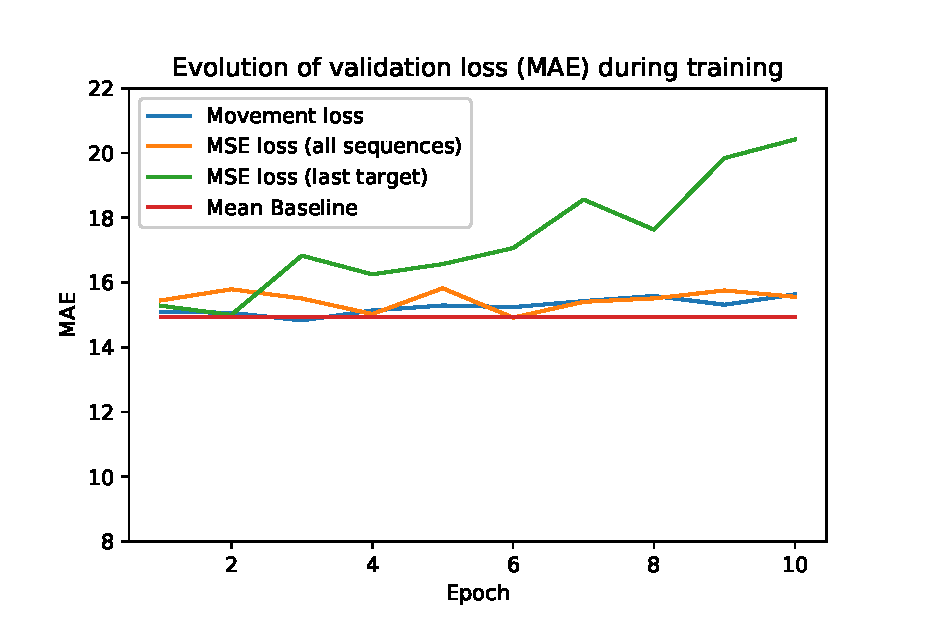
\includegraphics[width=0.95\linewidth]{training_evolution.eps}
	\end{center}
	\caption{Comparison of the different losses and the mean baseline}
	\label{fig:loss}
\end{figure}

This results might seem disappointing. Yet, the MAE is a mean and if we look closer we have some really good predictions for some articulations. For instance, figure \ref{wrist} shows the prediction of the wrist angle on the validation set. The prediction of certain articulations lower considerably our results, such as the prediction of the articulation shown in \ref{foire}

\begin{figure}[t]
	\begin{center}
		%\fbox{\rule{0pt}{2in} \rule{0.9\linewidth}{0pt}}
		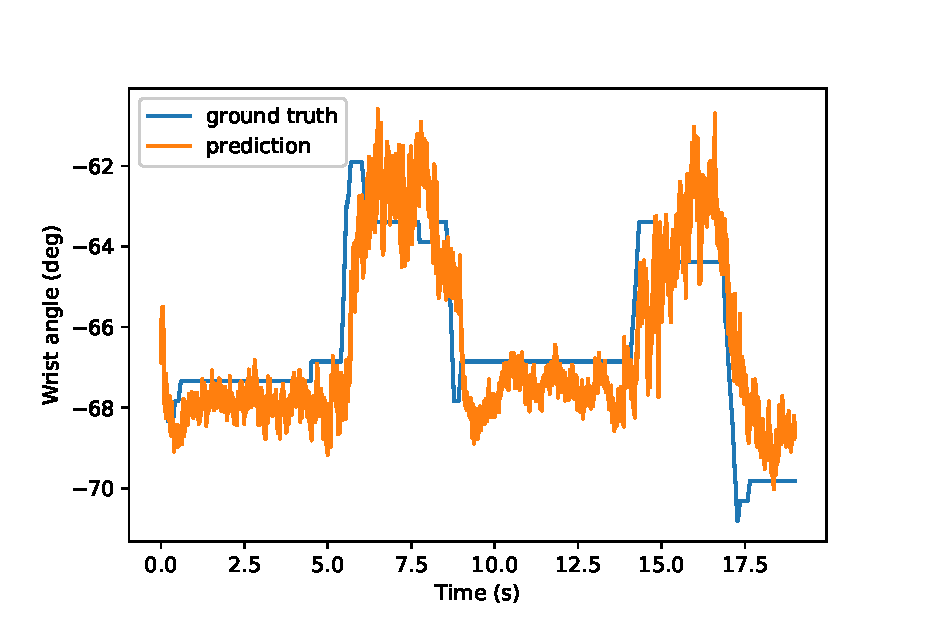
\includegraphics[width=0.95\linewidth]{wrist}
	\end{center}
	\caption{Prediction of the wrist angle on the validation set}
	\label{wrist}
\end{figure}

\begin{figure}[t]
	\begin{center}
		%\fbox{\rule{0pt}{2in} \rule{0.9\linewidth}{0pt}}
		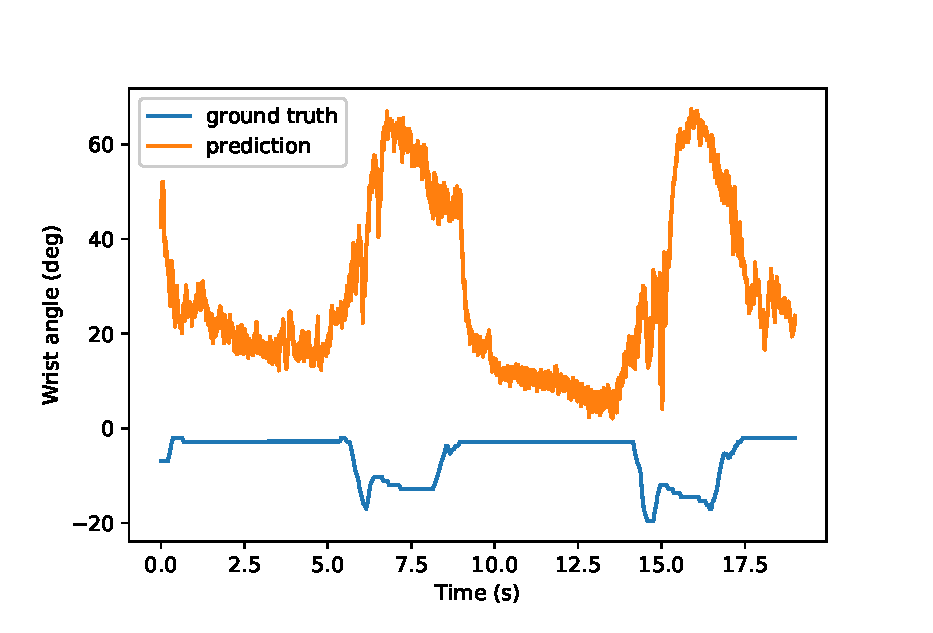
\includegraphics[width=0.95\linewidth]{foire.eps}
	\end{center}
	\caption{Prediction of a thumb angle on the validation set}
	\label{foire}
\end{figure}

Due to lack of time we did not manage to train and test a network on the same subjects but on different moments, but we expect this to improves the results and match those of \cite{Koch}. We try to finetune a model on a single subject by splitting its exercises. It improves the results up a MAE of 12.3. It is beyond the scope of our work, but it explains some of the results of the literature. 

\section{Conclusion}
%Presentation 10%; Style and writing 10%
In this project we have implemented the regression approach from predicting hand gestures from sEMG signals. A literature review encourage us to implement recurrent neural networks to solve this task, using the Ninapro database. We develop a methodology with the following steps : 
\begin{itemize}
    \item Database splitting 
    \item Sub-sampling
    \item Standardization
    \item Training neural networks :
    \subitem - with different architecture (LSTM, GRU)
    \subitem - with different loss we specifically design for this application
    \item Visualization and validation of the results
\end{itemize}
For each step listed, we implemented several experimentations (some have not been discussed here, only the more relevant have been kept). The conclusion of our work is that indeed this issue can be addressed with recurrent neural networks but methodology need to be improved to match state-of-the art approaches. For instance we strongly advise to compare results to the mean baseline and to try to understand what we are learning. As we show we struggled to reach this baseline on new subjects. It seems that it is hard to generalize the predictions. Thus fine-tuning on specific subject seems interesting but would be hard to do for amputee subjects.


{\small
\bibliographystyle{plain}
\bibliography{biblio}
}

\end{document}
